\documentclass[11pt,a4paper,oneside]{mwart}

\usepackage[utf8]{inputenc}

\def \MYHEADER {Projekt Zespołowy}
\def \MYTITLE {Projekt systemu do dystrybucji paliw płynnych}
\def \MYPDFTITLE {Cysterny}

\def \MYPDFDATE {\today}

\def \MYAUTHOR {\emph{Autorzy:}\\Tomasz \textsc{Bartnik}\\Jakub \textsc{Chrzanowski}\\Alexander \textsc{Dyszy}\\Aleksandra \textsc{Grzelak}}
\def \MYPDFAUTHOR {Aleksandra Grzelak}

\def \MYLECTURER {\emph{Prowadzący:} \\dr~hab.~in\.z.~C.~\textsc{Smutnicki}}

\def \MYLSTSETLANGUAGE {python}

\def \MYLSTSETFRAME {lines}
						%none, %single, 

\def \MYLSTSETKEYWORDS {} 

%konfiguracja bez treści, aby podłączać do innych plików

\usepackage[OT4,plmath,MeX]{polski}


\usepackage{indentfirst} % polski zwyczaj dla wciec akapitowych
\usepackage{graphicx}
%\usepackage[decimalsymbol=comma]{siunitx}
\usepackage{url}
\usepackage{pdflscape} 
\usepackage{subfigure}

\usepackage{wrapfig}
\usepackage[top=2cm, bottom=2cm, left=2.25cm, right=2.25cm]{geometry}

%\oddsidemargin 0.5cm
%\evensidemargin -0.5cm
\usepackage{algorithmic}
\usepackage[Algorytm]{algorithm}
\usepackage{listings}
\renewcommand{\labelitemi}{$\circ$}
\renewcommand{\today}{\oldstylenums{\number\day}~\ifcase\month\or
  stycznia\or lutego\or marca\or kwietnia\or maja\or czerwca\or
  lipca\or sierpnia\or września\or października\or
  listopada\or grudnia\fi \space\oldstylenums{\number\year} r.}

\usepackage{caption}
\usepackage{color}
\usepackage{rotating}
\usepackage{floatflt}
\usepackage{float}
\newfloat{scheme}{pb}{htbp} % second argument was {plt}
\floatname{scheme}{Schemat}
\newfloat{plot}{pb}{htbp} % second argument was {plt}
\floatname{plot}{Wykres}
\renewcommand*{\figurename}{Rysunek}
\renewcommand*{\tablename}{Tabela} 
\renewcommand*{\lstlistingname}{Kod}
\captionsetup{labelsep=period}
\usepackage{lscape}

\usepackage{amsmath}
\usepackage{mathtools}

\definecolor{dkgreen}{rgb}{0,0.5,0}
\definecolor{dkblue}{rgb}{0,0,0.7}
\definecolor{gray}{rgb}{0.5,0.5,0.5}
\definecolor{ltgray}{rgb}{0.8,0.8,0.8}
\definecolor{mauve}{rgb}{0.58,0,0.82}
\definecolor{maroon}{rgb}{0.5,0,0}

\newcommand{\HRule}{\rule{\linewidth}{0.5mm}}
\newcommand{\linia}{\rule{\linewidth}{0.1mm}}

\usepackage[ 
	pdftitle=\MYPDFTITLE,
	pdfauthor=\MYPDFAUTHOR,
	bookmarks=true, 
	bookmarksnumbered=true, 
	unicode=true, 
	pdftex, 
	pdfnewwindow=true,
	colorlinks=true,
	linkcolor=blue,
	hidelinks
]{hyperref} 


\lstset{
	language=\MYLSTSETLANGUAGE,
	frame=\MYLSTSETFRAME,
	morekeywords=\MYLSTSETKEYWORDS,
	basicstyle=\footnotesize,
	numbers=left, 
	numberstyle=\tiny\color{gray},
	stepnumber=1,
	columns=fixed,
	numbersep=20pt, 
	backgroundcolor=\color{white}, 
	showspaces=false, 
	showstringspaces=true, 
	showtabs=false, 
	rulecolor=\color{ltgray},
	tabsize=4,
	breakatwhitespace=true,
	breakindent=30pt,
	breaklines=true,
	breakautoindent=true,
	prebreak=\mbox{{\color{red}$\hookleftarrow$}},
	postbreak=\mbox{{\color{red}$\hookrightarrow$}}\space,
	keywordstyle=\color{dkblue},
	commentstyle=\color{red},
	stringstyle=\color{dkgreen},
	identifierstyle=\color{maroon},
	morekeywords=_MY_MACRO_LSTSET_KEYWORDS
}


%\renewcommand{\thefootnote}{_MY_MACRO_FOOTNOTE}
%define _MY_MACRO_FOOTNOTE $\dagger$
						  %\fnsymbol{footnote}
						  % $\bullet${}
						  %\Roman{footnote}
						  %\alph{footnote}


\usepackage{float}
%\newfloat{schemat}{pb}{htpb} % second argument should be {htbp} in your actual iedocument
%\floatname{schemat}{Schemat}
\usepackage{pdfpages}

%\newfloat{wykres}{pb}{htpb} % second argument should be {htbp} in your actual document
%\floatname{wykres}{Rys.}

\usepackage{tocbasic}
\DeclareNewTOC[%
  type=schemat,%
  types=schems,% used in the \listof.. command
  float,% define a floating environment
  floattype=4,% see below
  name=Schemat,%
  listname={Spis schematów}%
]{lop}

\DeclareNewTOC[%
  type=wykres,%
  types=wykress,% used in the \listof.. command
  float,% define a floating environment
  floattype=4,% see below
  name=Rys.,%
  listname={Spis rysunków}%
]{lor}



\newcommand{\itab}[1]{\hspace{0em}\rlap{#1}}
\newcommand{\tab}[1]{\hspace{.29\textwidth}\rlap{#1}}


\renewcommand\algorithmicforall{\textbf{Dla wszystkich}}
\renewcommand\algorithmicfor{\textbf{Dla}}
\renewcommand\algorithmicdo{\textbf{wykonaj:}}
\renewcommand\algorithmicendfor{\textbf{Koniec.}}
\renewcommand\algorithmicif{\textbf{Jeżeli}}
\renewcommand\algorithmicthen{\textbf{to:}}
\renewcommand\algorithmicendif{\textbf{Koniec.}}
\renewcommand\algorithmicelse{\textbf{W przeciwnym wypadku:}}
\renewcommand\algorithmicwhile{\textbf{Dopóki}}
\renewcommand\algorithmicendwhile{\textbf{Koniec.}}
\renewcommand\algorithmicreturn{\textbf{Zwróć}}
\setlength{\algorithmicindent}{2em}


\begin{document}

\begin{titlepage}
\begin{center}
\textsc{\Large \MYHEADER }\\[3cm]
\centering{\HRule \\[0.5cm]}
{\LARGE  \textsc{ \MYTITLE }\\[0.4cm]}
\centering{\HRule \\[1.5cm]}
\begin{minipage}[b]{0.4\textwidth}
\begin{flushleft} \large
\MYAUTHOR
\end{flushleft}
\end{minipage}
\begin{minipage}[b]{0.4\textwidth}
\begin{flushright} \large
\MYLECTURER
\end{flushright}
\end{minipage}
\vfill
{\large \MYPDFDATE}
\end{center}
\end{titlepage}


\newpage
\thispagestyle{empty}
\newpage

\setcounter{tocdepth}{3}
\tableofcontents
\newpage


% =============================================
\section{Cel projektu}
Zaprojektować system do dystrybucji paliw płynnych za pomocą floty cystern samochodowych w oparciu o zasoby paliw zgromadzone w jednej centralnej bazie (magazynie).

%system do dystrybucji paliw płynnych za pomocą floty cystern samochodowych w oparciu o zasoby paliw zgromadzone w jednej centralnej bazie
% =============================================
\section{Założenia projektowe}
Dostęp do systemu jest realizowany za pomocą standardowej przeglądarki. Zamówienia na paliwa (ich rodzaj i ilość), kategorie cystern dostępne w bazie transportowej, odległości transportowe, ograniczenia czasu pracy kierowców, etc., są kolekcjonowane w bazie danych serwera zaś zarządzanie nimi odbywa się poprzez aplikację webową. Zamówienia są składane on-line przez lokalne stacje paliw i realizowane wg przyjętego scenariusza obsługi. Algorytm optymalizacyjny jest uruchamiany na serwerze.

System zawiera 4 moduły: 
\begin{itemize}
  \item baza danych z aplikacją serwera plus webowa aplikacja zamówień na dostarczenie paliw, 
  \item algorytm optymalizacji tras cystern i polityki ich ładowania/rozładowania, 
  \item interfejs graficzny systemu, 
  \item system wizualizacji mapy transportowej.
\end{itemize}


 % ==== TODO ======
\section {Koncepcja rozwiązania}

Algorytm realizujący postawione zadanie rozwiązuje dwa cele. Optymalizuje dobór cystern wraz z rozmieszczeniem paliwa w ich komorach według wybranego kryterium, minimalizuje ilość użytych pojazdów oraz dąży do minimalizacji czasu pracy cystern, a tym samym kosztów zużytego paliwa. Podczas rozwiązywania problemu brany pod uwagę jest także maksymalny czas pracy kierowcy.

Polityka realizacji zamówień działa w systemie sesyjnym. To znaczy, że zamówienia nadchodzące danego dnia uszeregowane zostają o ustalonej godzinie dnia następnego. Zamówienia pojawiające się po owej godzinie podlegają szeregowaniu następnego dnia.

\subsection{Stategia wyboru cystern}

	Pod uwagę brane były dwie strategie wyboru cystern. Pierwsza, tzw. Biggest-Tank-First polega na wybieraniu do obsługi zamówienia zawsze cysterny o największej pojemności. Takie podejście ma na celu zminimalizowanie ilości użytych pojazdów kosztem wydłużenia trasy jaką pojazd musi przebyć. Drugą strategią jest strategia Fittest-Tank-First, opierająca się o próby doboru takich cystern, których pojemności są jak najbardziej zbliżone do rozmiaru zamówienia. Stosując tą trategię zmniejszamy sumaryczną odległość przebytą przez pojedynczą cysternę jednocześnie zwiększając ilość użytych do wykonania zleceń pojazdów. W niniejszym projekcie zdecydowano sięna przyjęcie strategii pierwszej, a więc Biggest-Tank-First.

  \subsection{Strategia wypełniania komór cystern paliwem.}

	Podczas napełniania komór cystern brane są pod uwagę różne czynniki. W przypadku, gdy ilość zamówionego paliwa jest większa od pojemności rozpatrywanej komory, wówczas komora ta zostanie napełniona, a pozostała część zamówionego paliwa przekazana zostanie do kolejnej komory. Jeśli podczas wyboru komory dla danej ilości paliwa pojemność tej komory jest większa niż ilość paliwa, wówczas poszukiwany jest zbiornik mniejszy, o pojemności jak najbardziej zblizonej do rozmiaru rozpatrywanego zamówienia. Pozwala to uniknąć wypełniania dużych komór małymi ilościami paliwa, co ma wpływ na koszty transportu, a także jego bezpieczeństwo. 

  \subsection{Ograniczenie związane z maksymalnycm czasem pracy kierowcy}
	Odległości między punktami rozlewu paliwa określone są czasem potrzebnym do przebycia drogi między nimi. Podczas realizacji poprzednio opisanych zadań przeprowadzana jest estymacja czasu potrzebnego do zrealizowania zadania. Realizowane jest to w następujący sposób. Podczas wyboru cysterny do zrealizowania zadania wyliczany jest pozostały czas możliwej pracy kierowcy owego pojazdu na podstawie z góry ustalonego maksymalnego czasu dziennej pracy oraz przybliżonego czasu wykonania zadań już do cysterny przydzielonych. W przypadku wyznaczenia sumarycznego czasu pracy przekraczającego maksymalny, cysterna nie jest brana pod uwagę do tego zamówienia.


\subsection{Inne algorytmy użyte w realizacji rozwiązywania problemu}
	Do wyznaczenia najkrótszych tras pomiędzy węzłami użyto algorytm Dijkstry.

	Realizuje on operacje szukania najkrótszych ścieżek w grafie. Użyty graf jest ważonym grafem nieskierowanym. Działanie tego algorytmu stanowi również podstawę do estymacji "w locie" czasu wykonania kolejnego nałozonego na cysternę zadania.	Wynikowy czas jest nie większy niż rzeczywisty czas realizacji.

  \subsection{Dalszy rozwój algorytmu}

	W przypadku dalszego rozwoju opisanego wyżej algorytmu należałoby zaopatrzyć go w możliwość doboru cystern według drugiego kryterium. Ponadto dodatkową minimalizację kosztów transportu paliwa można uzyskać rozwiązując problem plecakowy dla każdej cysterny, po wykończeniu jej pozostałego czasu pracy. Po odzyskaniu dodatkowego czasu związanego z kolejną optymalizacją trasy cysterny, pojazd mógłby zostać przywrócony do kolejki cystern rozpatrywanych w realizacji zamówień. Spowodowałoby to jednak gwałtowny wzrost złożoności obliczeniowej algorytmu i jego modyfikacja w tym kierunku byłaby sensowna jedynie w przypadku stosunkowo niewielkiej ilości punktów obsługiwanych przez system.


 
\section{Użyte narzędzia}
Do stworzenia aplikacji internetowej wraz z bazą danych użyto platformy \textsc{Django}, dostępnej na licencji \textsc{bsd}\footnote{dostępne w Internecie: \url{https://www.djangoproject.com/}}. Pozwala ona na tworzenie złożonych stron internetowych, opartych na bazie danych. Opiera się na wzorcu projektowym podobnym do model-widok-kontroler (model-view-template). Pozwala na oddzielenie logiki aplikacji (widok), logiki biznesowej (model), wyglądu (szablon) oraz bazy danych.

Jako system zarządzania bazą danych został wybrany \textsc{SQLite}. System ten przetrzymuje bazę danych w jednym pliku binarnym.
SQLite obsługuje zapytania zagnieżdzone, klucze obce, transakce, przechowywanie baz danych w pamięci RAM komputera, co przyspiesza działanie bazy.

\section{Szczegółowy opis rozwiązania}
 
\paragraph{Organizacja danych wejściowych}
\begin{enumerate}
  \item Zamówienia (Orders) - zamówienie złożone na kilka różnych rodzajów paliwa traktowane jest jak kilka różnych zamówień. Z punktu widzenia algorytmu znaczenie mają takie parametry zamówienia jak ilość zamówionego paliwa i destynacja.

  \item Cysterny (Tanks) - Głównymi parametrami cystern mającymi znaczenie w pracy algorytmu są sumaryczna pojemność, rozkład komór, maksymalny/pozostały czas pracy, oraz tzw, lokalizacja. Ten ostatni parametr stanowi podstawę do estymacji czasu wykonania potencjalnego zadania. Przyjmuje się, że komory  w cysternie posortowane są nierosnąco.


  \item Węzły (Nodes) - Punkty rozlewu paliwa mające ścisły związek z zamawiającymi. Przedstawione są za pomocą grafu nieskierowanego z wagami odpowiadającymi czasowi przebycia drogi między poszczególnymi węzłami.

\end{enumerate}

Ideę działania algorytmu opisuje algorytm~\ref{alg:opt}.

\begin{algorithm}[htbp]
  \caption{Algorytm wyboru zbiorników oraz cystern do realizacji zadań.}
  \label{alg:opt}
  \begin{algorithmic}
    \STATE {Posortuj \emph{zamówienia} po ilości paliwa nierosnąco.}
    \STATE {Posortuj \emph{cysterny} według kryterium Biggest-Tank-First niemalejąco.}
    \WHILE {istnieją nie zrealizowane zamówienia:}
    \STATE {wybierz największe nieobsłużone zamówienie \emph{order}, $\quad$ (1)}
    \STATE {wybierz cysternę \emph{tank} najlepiej odpowiadającą kryterium, $\quad$ (2)}
    \IF { \emph{tank} posiada komory \emph{cells} niezapełnione \textbf{oraz} pozostały czas pracy jest mniejszy bądź równy od czasu realizacji zamówienia \emph{order}}
    \IF { \emph{order} jest niezrealizowane (lub jest tylko częściowo), $\quad$ (3)}
    \STATE {wybierz największą niezapełnioną komórkę cysterny \emph{cell}  }
          \IF{ pojemność \emph{cell} jest mniejsza bądź równa od rozmiaru zamówienia \emph{order}}
            \STATE { wypełnij komorę \emph{cell} częścią zamówieniea \emph{order}}
        \ENDIF
        \IF{ \emph{tank} nie posaida wolnych komór}
          \STATE { idź do (2)}
          \ELSE 
          \STATE { idź do (3)}
        \ENDIF
       \ELSE
       \STATE { idź do (1)}
      \ENDIF
     \ELSE
     \STATE { idź do (2)}
    \ENDIF

    \ENDWHILE
  \end{algorithmic}
\end{algorithm}

%1. SORTUJ zamówienia po ilości paliwa nierosnąco
%2. SORTUJ cysterny według wybranego kryterium (Biggest-Tank-First) niemalejąco
%3. DOPÓKI istnieją zamówienia nie zrealizowane:
%4.		WYBIERZ największe nieobsłużone zamówienie <ORDER>
%5.		WYBIERZ cysternę <TANK> najlepiej odpowiadającą kryterium
%6.		JEŚLI <TANK> posiada komory<CELLS> niezapełnione ORAZ pozostały czas pracy <= czas realizacji <ORDER>:
%7.			JEŚLI <ORDER> jest niezrealizowane (lub tylko częściowo):
%8.				WYBIERZ największą niezapełnioną komórkę cysterny<CELL>
%9.				JEŚLI pojemność <CELL> <= rozmiar <ORDER>
%10.					WYPELNIJ komorę <CELL> częścią zamówienia <ORDER>
%11.				JEŚLI <TANK> nie posiada wolnych komór
%12.					IDŹ DO kroku 5.
%13.				W PRZECIWNYM PRZYPADKU
%14.					IDŹ DO kroku 7.
%15.			W PRZECIWNYM PRZYPADKU
%16.				IDŹ do kroku 4.
%17.		W PRZECIWNYM PRZYPADKU
%18.			IDŹ do kroku 5.
%19. KONIEC

\section{Opis techniczny oprogramowania}
\subsection{Architektura}
Architektura systemu jest modłuowa. System składa się z interfejsu \textsc{www}, aplikacji zarządzającej, bazy danych oraz algorytmu optymalizacjynego.

Przepływ informacji w systemie został przedstawiony na obrazku \ref{fig:informacja}. Użytkownik poprzez interfejs www ma możliwość wglądu w stan realizacji zamówień, trasę i załadunku cystern. Jednocześnie poprzez stronę może składać nowe zamówienie. Żądania użytkownika są kierowane do aplikacji, która je obsługuje. Nowe zamówienie jest zapisywane w bazie danych. Z bazy jest pobierana informacja o pozostałych zamówieniach i stanie floty cystern. Te informacje przekazywane są poprzez aplikacje do algorytmu optymalizującego, który na tej podstawie wylicza załadunek i optymalną trasę cystern.  Nowy stan jest uaktualniany w bazie i wizualizowany użytkownikowi.
Administrator ponadto ma możliwość pełnego wglądu do bazy danych i jej modyfikacji.

\begin{schemat}
  \centering
  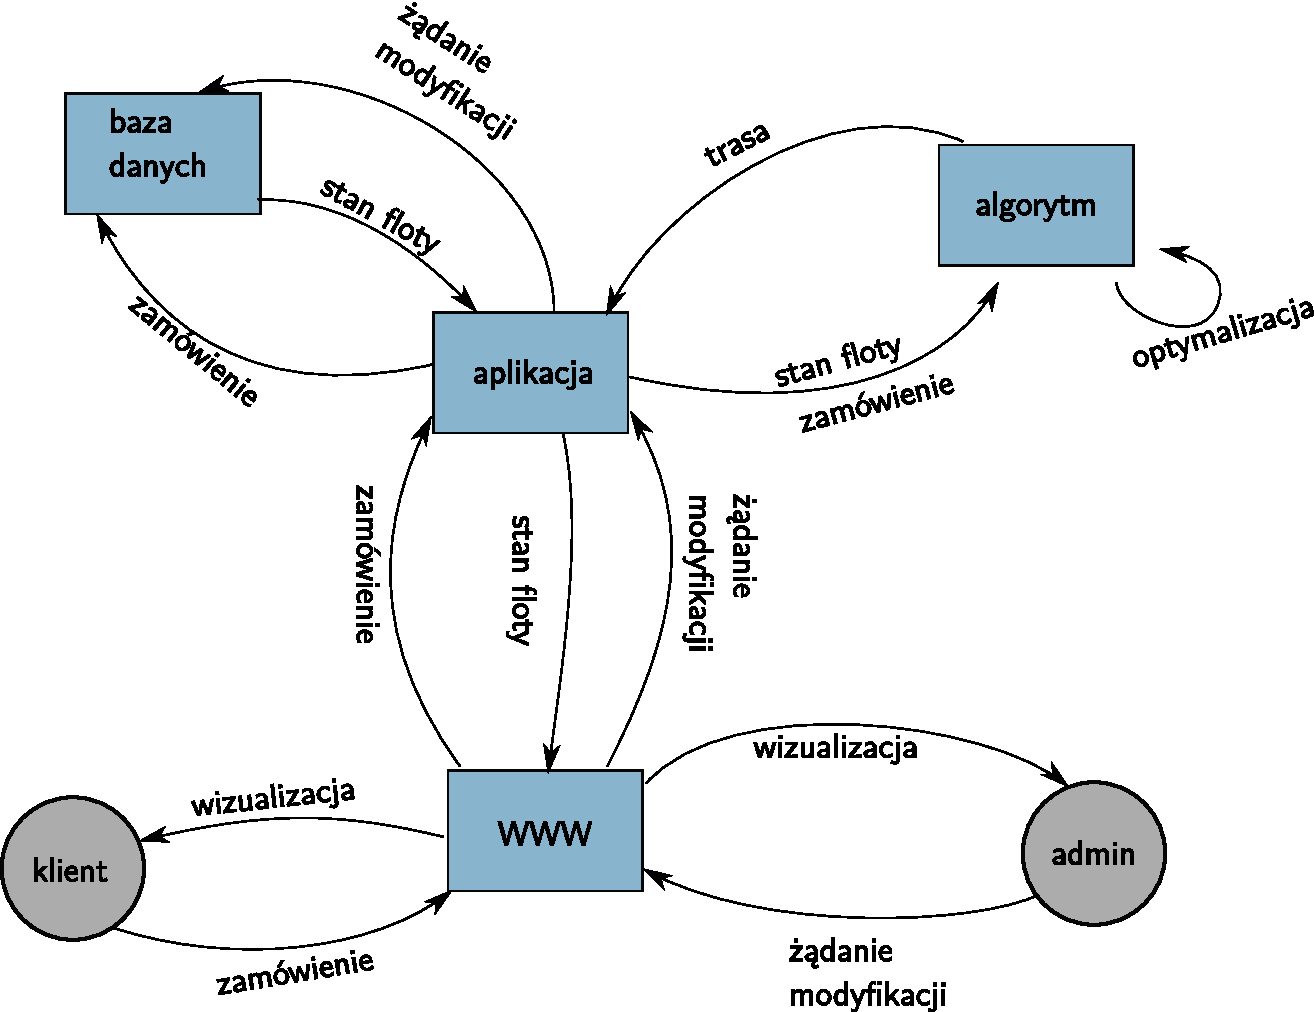
\includegraphics[width=0.6\textwidth]{pics/przep_inf.pdf}
  \caption{Przepływ informacji w systemie.}
  \label{fig:informacja}
\end{schemat}

 % ==== TODO ======
\subsection{Baza danych}
Baza danych oparta jest o modele:
\begin{itemize}
  \item \emph{Paliwo} (Fuel) 
    \begin{itemize}
      \item typ paliwa (np. Pb95),
    \end{itemize}
    \item \emph{Kontener} (Container) 
          \begin{itemize}
            \item typ paliwa jaki jest wewnątrz (jeżeli jest)
            \item maksymalna pojemność
            \item do której cysterny należy
            \item przydzielone zamówienie (jeżeli jest)
    \end{itemize}
      \item \emph{Cysterna} (Cistern) 
            \begin{itemize}
      \item nazwa cysterny,
      \item status (czy jest w trasie)
      \item pozostały czas pracy,
      \item ostanie odwiedzone miasto,
    \end{itemize}
    \item \emph{Miasto} (City)
          \begin{itemize}
      \item nazwa miasta
    \end{itemize}
    \item \emph{Zamówienie} (Order) 
    \begin{itemize}
      \item miasto docelowe,
      \item zamówione paliwo
      \item ilość paliwa
      \item status realizaji
      \item data złożenia zamówienia
    \end{itemize}
    \item \emph{Status zamówienia} (OrderStatus) 
    \begin{itemize}
      \item gotowe / w trakcie realizacji / zrealizowane
    \end{itemize}
    \item \emph{Odległość} (CityDistiance) -- miasta i odległości między nimi,
    \begin{itemize}
      \item miasto początowe
      \item miasto końcowe
      \item odległość między nimi
    \end{itemize}
    \item \emph{Ścieżka} (Path) 
    \begin{itemize}
      \item cysterna,
      \item miasta do odwiedzenia (odległość),
    \end{itemize}
\end{itemize}

\begin{schemat}
  \centering
  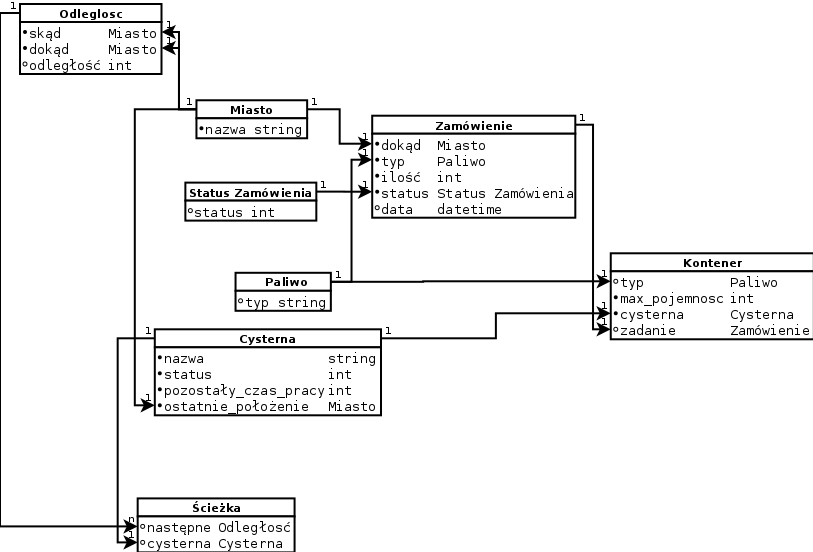
\includegraphics[width=0.65\textwidth]{pics/baza.png}
  \caption{Baza danych w aplikacji.}
  \label{fig:baza}
\end{schemat}

 % ==== TODO ======
\subsection{Aplikacja www}
Aplikacja bazuje na widokach (logika aplikacji) oraz szablonach (uzupełnianych przez aplikację).  

 % ==== TODO ======
\subsection{Wizualizacja tras}

  Do wizualizacji trasy wykorzystana została funkcjonalność dostarczana przez Google Maps. 
%System wizualizacji bazuje na komunikacji na Google Maps. Dane z bazy dotyczące trasy i położenia cystern są konwertowane i wyświetlane za pomocą apletu. 

  Na podstawie wpisów z bazy danych, w szablonie strony generowany jest JavaScript umożliwiający wizualizację tras przejazdu cystern.

\subsection{Interfejs użytkownika}
Po uruchomieniu aplikacji na serwerze, należy wpisać odpowiedni adres w przeglądarkę. Powinna pojawić się strona główna (rys.\ref{fig:index}).

\begin{wykres}[htbp]
  \centering
  \begin{tabular}{c}
    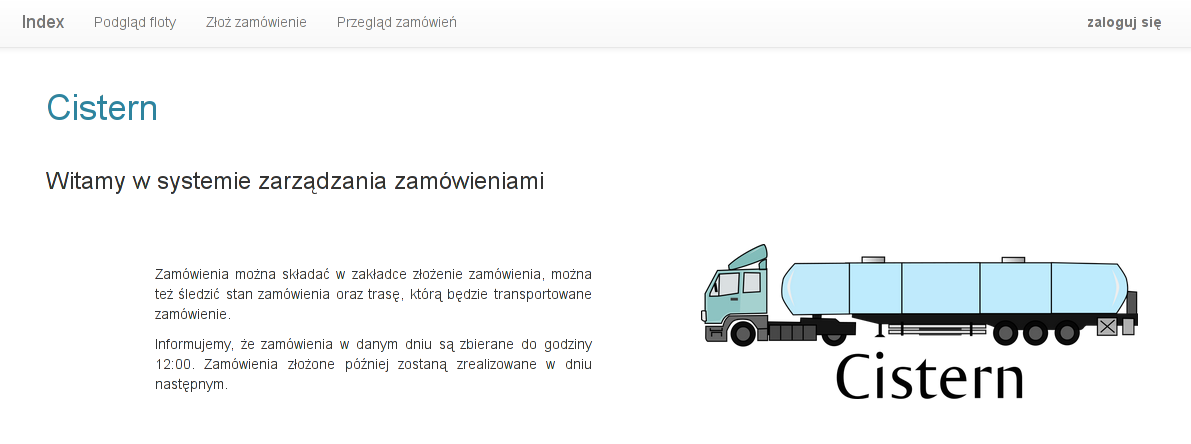
\includegraphics[width=0.99\textwidth]{pics/after_login.png} \\
    \raisebox{1.5ex}{a) Widok strony głównej użytkownika niezalogowanego.} \\
    \\
    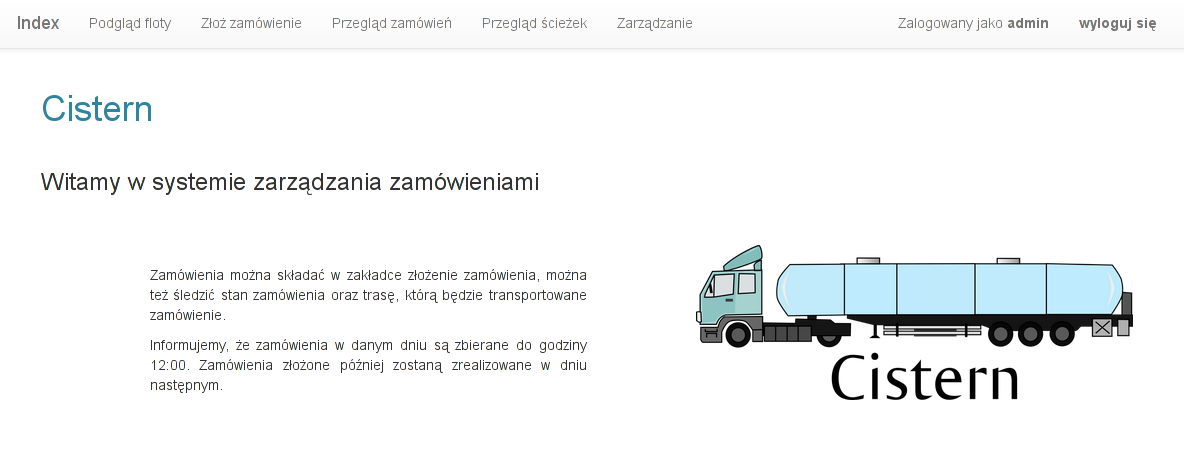
\includegraphics[width=0.99\textwidth]{pics/index.png} \\
  \raisebox{1.5ex}{b)  Widok strony głównej po autoryzacji.}\\ 
\end{tabular}
  \caption{Strona główna.}
  \label{fig:index}
\end{wykres}

Nie będąc zalogowanym, można przejść do zakładek: składnie zamówień, przegląd zamówień, przegląd cystern oraz do panelu logowania (rys.\ref{fig:index}a). 

W przypadku zalogowanych użytkowników możliwe jest również przejście do panelu zarządzania i przegląd tras cystern oraz wylogowanie (rys.~\ref{fig:index}b).

\subsubsection{Logowanie}
Aby zabezpieczyć system przed niepowołanym dostępem, konieczne jest posiadanie uprawnień przy dokonywaniu modyfikacji systemu, w tym też uruchamianie algorytmu optymalizującego. W przypadku przejścia na taką stronę (np. poprzez wpisanie adresu) bez uwierzytelnienia, pojawi się okno logowania (rys.~\ref{fig:login}). 

\begin{wykres}[htbp]
  \centering
  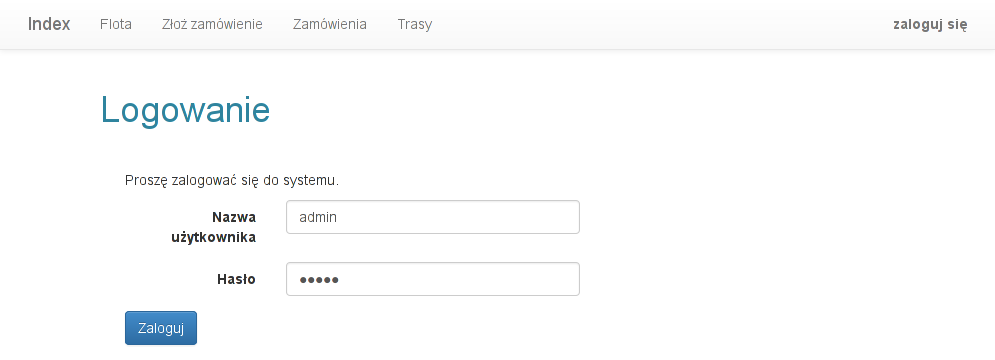
\includegraphics[width=0.99\textwidth]{pics/login.png}
  \caption{Widok logowania.}
  \label{fig:login}
\end{wykres}


\subsubsection{Przeglądanie zgłoszeń}
W zakładce \emph{Przeglądanie zgłoszeń}, można zobaczyć listę zamówień (rys.~\ref{fig:order}a). Po kliknięciu w id zamówienia (data złożenia zamówienia), przechodzi się w szczegóły zamówienia, gdzie wyświetlane są: gdzie ma być dostarczone zamówienie, data, ilość i typ paliwa oraz cysterny obsługujące zlecenie (rys.~\ref{fig:order}b). Po kliknięciu w nazwę cysterny można przejść do szczegółów cysterny.
\begin{wykres}[htbp]
  \centering
  \begin{tabular}{c}
    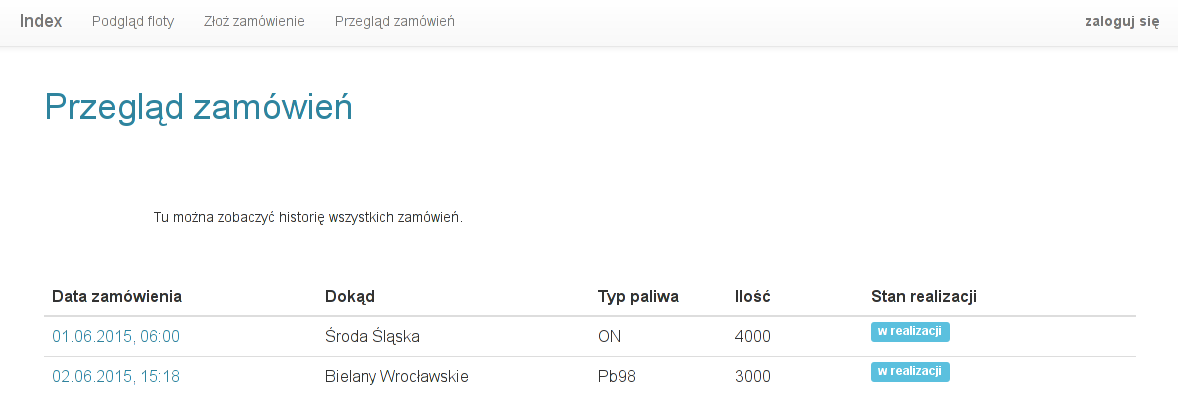
\includegraphics[width=0.99\textwidth]{pics/order_list.png} \\
    \raisebox{1.5ex}{a) Przeglądanie zamówień.} \\
    \\
    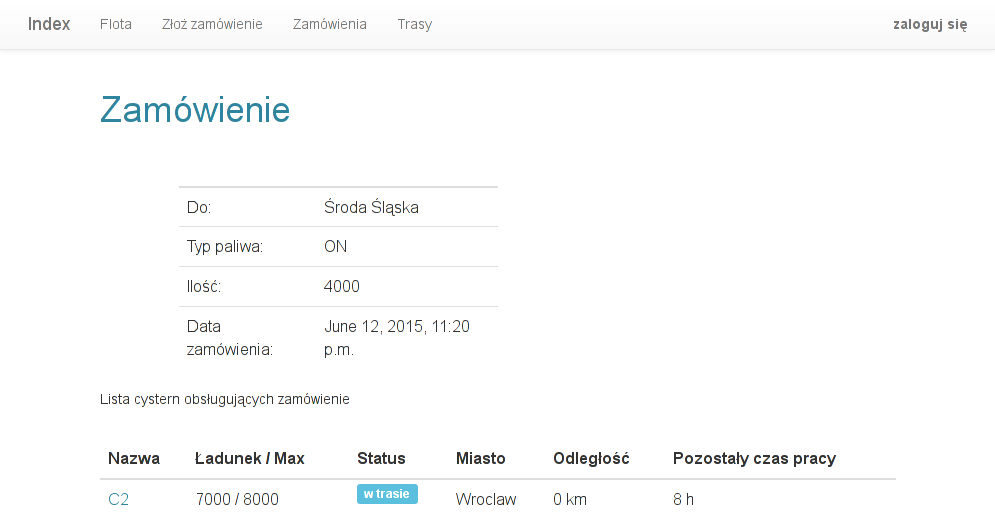
\includegraphics[width=0.99\textwidth]{pics/order_detail.png} \\
  \raisebox{1.5ex}{b) Szczegóły zamówienia.}\\ 
\end{tabular}
  \caption{Przeglądanie zgłoszeń.}
  \label{fig:order}
\end{wykres}

\subsubsection{Przeglądanie cystern}
W zakładce \emph{Przeglądania cystern}, pokazane są wszyskie cysterny, wraz z informacją czy realizuje ona zamówienie, pojemność całkowita i pojemność załadunku (rys.~\ref{fig:cistern}a). Po kliknięciu w nazwę cysterny, wyświetlane są szczegóły dotyczące cysterny: przegląd wszytkich kontenerów na paliwo wraz z zamówieniami jakie są im przydzielone, pojemność kontenera oraz typ przewożonego paliwa. Pokazana jest też trasa cysterny oraz podgląd cysterny (rys.~\ref{fig:cistern}b).

\begin{wykres}[htbp]
  \centering
  \begin{tabular}{cc}
    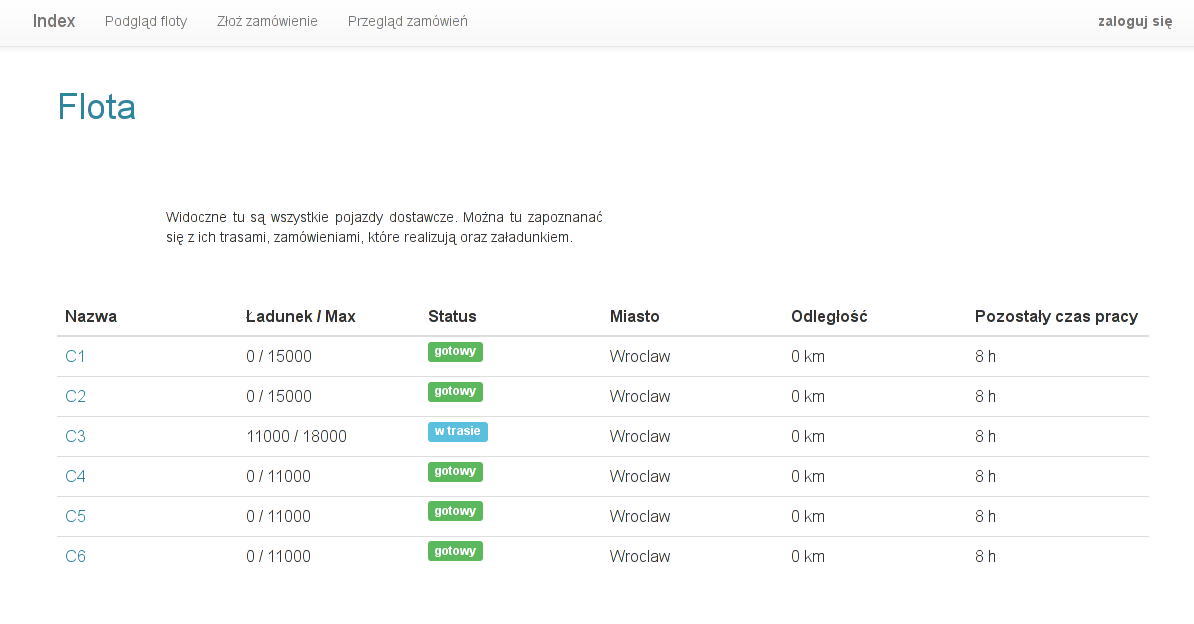
\includegraphics[width=0.99\textwidth]{pics/cistern_list.png} \\
    \raisebox{1.5ex}{a) Przeglądanie floty.} \\
    \\
    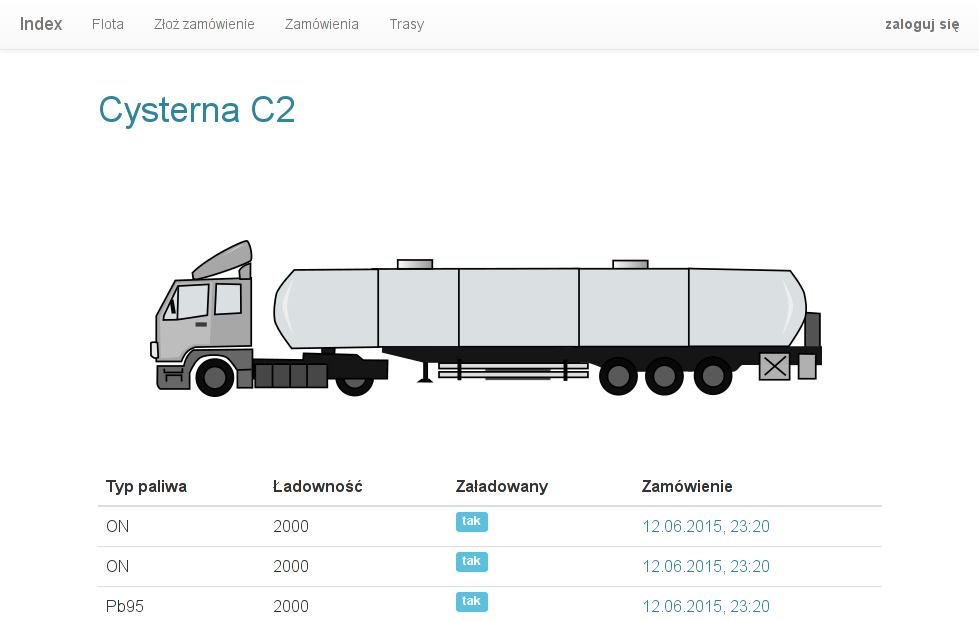
\includegraphics[width=0.99\textwidth]{pics/cistern_detail.png} \\
  \raisebox{1.5ex}{b) Szczegóły cysterny.}\\ 
\end{tabular}
  \caption{Przeglądanie cystern.}
  \label{fig:cistern}
\end{wykres}

\subsubsection{Dodawnie zgłoszeń}
W celu dodania zgłoszenia, należy przejść w zakładkę \emph{Złóż zamówienie}. Pojawia się formularz zgłoszeniowy, w którym należy wybrać miejsce docelowe, typ paliwa i ilość (rys.~\ref{fig:order_form}). Po pomyślnym przyjęciu zgłoszenia pojawia się komunikat i użytkownik przekierowywany jest na stronę główną.

\begin{wykres}[htbp]
  \centering
  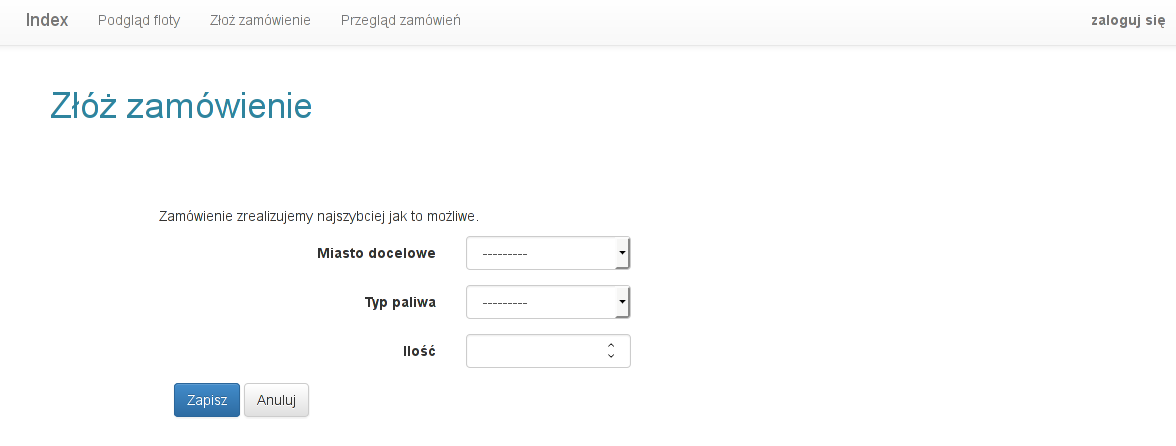
\includegraphics[width=0.99\textwidth]{pics/order_form.png}
  \caption{Formularz zamówienia.}
  \label{fig:order_form}
\end{wykres}

\subsubsection{Przeliczanie tras}
W przypadku, gdy użytkownik jest zalogowany, ma możlwość również ręcznego przeliczania trasy. Należy przejść w zakładkę \emph{Zarządzanie} i potwierdzić przeliczenie trasy (rys.~\ref{fig:manage}). Po przeliczeniu tras cystern, użytkownik zostanie przekierowany na stronę główną.
\begin{wykres}[htbp]
  \centering
  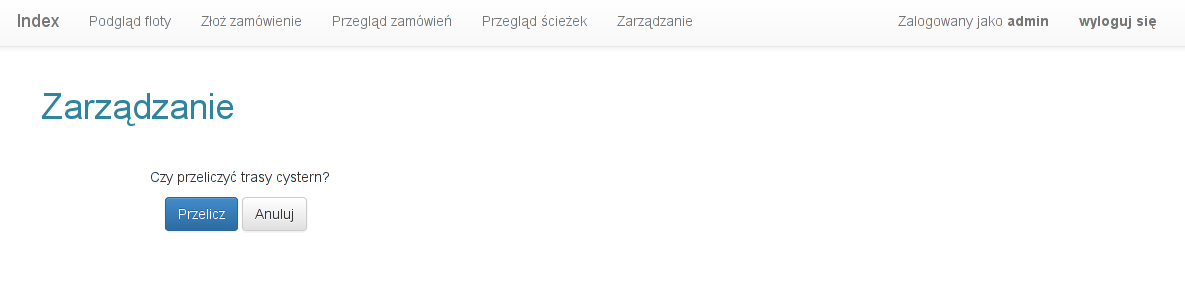
\includegraphics[width=0.99\textwidth]{pics/manage.png}
  \caption{Ręczne uruchomienie przeliczania tras.}
  \label{fig:manage}
\end{wykres}

\subsubsection{Podgląd ścieżek}
Zalogowany użytkownik ma możliwość również wglądu w obliczone trasy. W tym celu należy przejść w zakładkę \emph{Podgląd śćieżek}. Wyświetlą się szczegóły zaplanowanych tras (rys.~\ref{fig:path}).
\begin{wykres}[htbp]
  \centering
  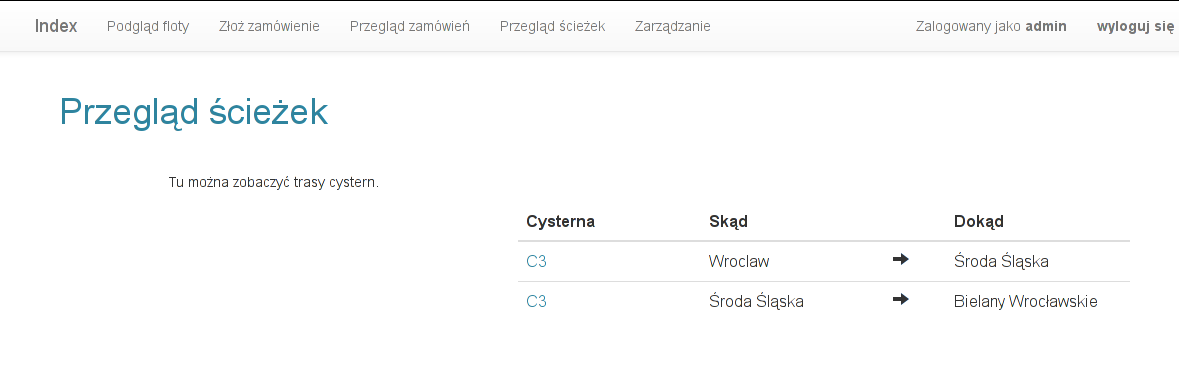
\includegraphics[width=0.99\textwidth]{pics/path.png}
  \caption{Podgląd tras cystern.}
  \label{fig:path}
\end{wykres}

\subsubsection{Panel administracyjny}
Aby mieć możliwość wglądu oraz modyfikacji zawartości bazy danych, należy przejść do \emph{Panelu administracyjnego}. Po wpisaniu w adres przeglądarki adresu oraz zalogowaniu się (rys.~\ref{fig:admin}a), można zobaczyć listę modeli bazy (rys.~\ref{fig:admin}b). Po wybraniu modelu, widoczna jest lista obiektów (rys.~\ref{fig:admin}c), jest możliwość dodania, modyfikacji lub usunięcia obiektu (rys.~\ref{fig:admin}d).

\begin{wykres}[htbp]
  \centering
  \begin{tabular}{cc}
    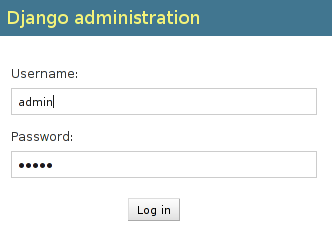
\includegraphics[width=0.5\textwidth]{pics/admin_login.png} &
    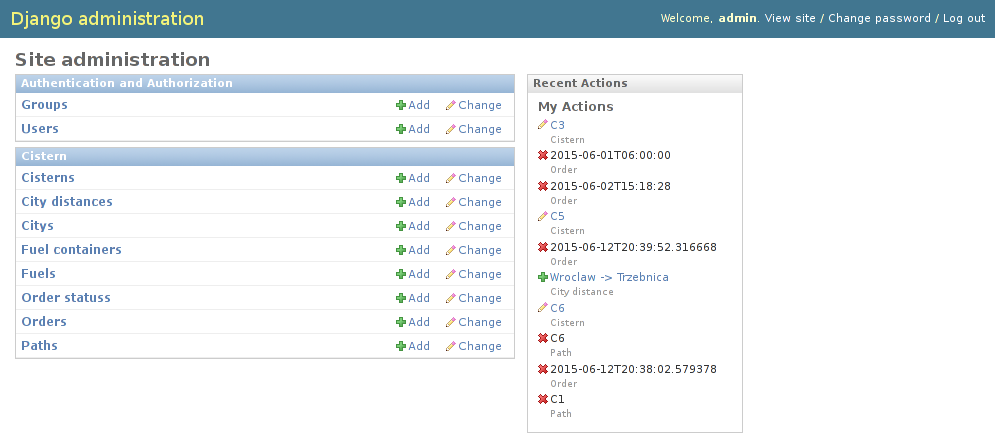
\includegraphics[width=0.5\textwidth]{pics/admin_all.png} \\
    \raisebox{1.5ex}{a) Okno logowania administratora.} &
  \raisebox{1.5ex}{b) Lista modeli w bazie danych.}\\ 
  \\
\end{tabular}
  \begin{tabular}{c}
    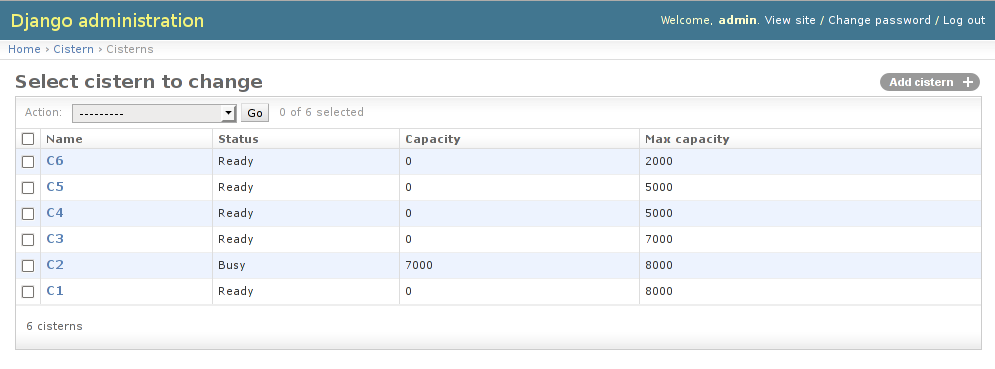
\includegraphics[width=0.99\textwidth]{pics/admin_list.png} \\
  \raisebox{1.5ex}{c) Przykładowa lista obiektów (cysterny).} \\ 
  \\
    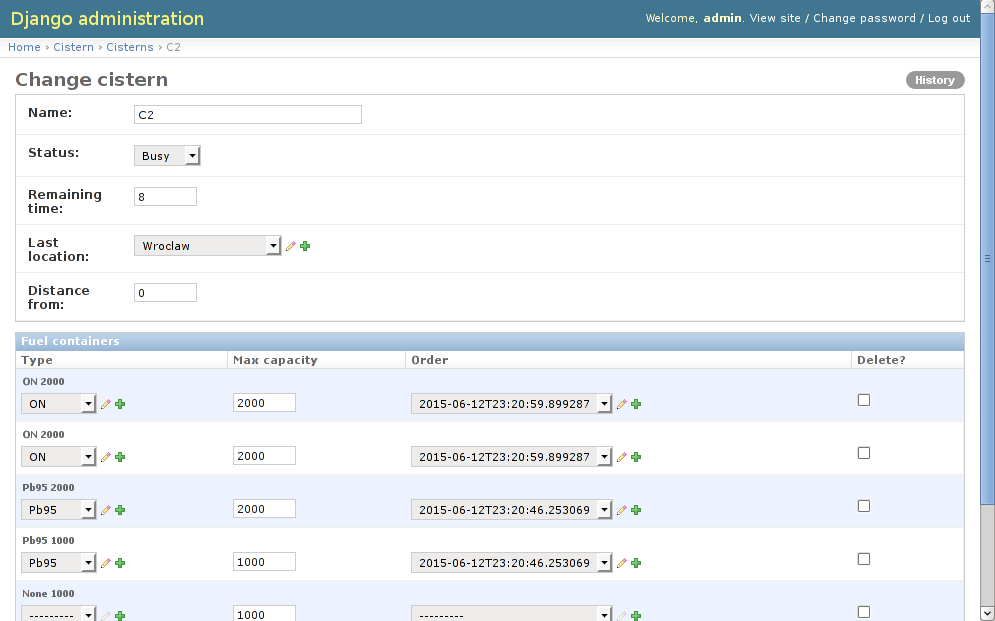
\includegraphics[width=0.99\textwidth]{pics/admin_detail.png} \\
  \raisebox{1.5ex}{d) Szczegółowy widok obiektu (cysterna).}\\ 
\end{tabular}
  \caption{Panel administracyjny.}
  \label{fig:admin}
\end{wykres}

 % ==== TODO ======
\section{Uwagi i wnioski}



 
 \newpage
 \listoftables
 %\listoffigures
 \listofwykress
 \listofschems

% =============================================
 \begin{thebibliography}{12}
   \bibitem{mgr} M. Bartecki \emph{System zarządzania dystrybucją paliw.} 
 \end{thebibliography}
\end{document}
